%source: http://www.fit.vutbr.cz/study/advisor/sablona_prezentace/FIT_novy_styl_4x3-EN-LaTeX.zip

\documentclass[10pt,xcolor=pdflatex]{beamer}
\usepackage{newcent}
\usepackage[utf8]{inputenc}
\usepackage[czech]{babel}
\usepackage{hyperref}
\usepackage{fancyvrb}
\usepackage{paralist}
\usepackage{enumitem}
\usetheme{FIT}

%%%%%%%%%%%%%%%%%%%%%%%%%%%%%%%%%%%%%%%%%%%%%%%%%%%%%%%%%%%%%%%%%%
\title[IAL projekt]{IAL projekt}
\subtitle{Varianta č.6 - Obarvení grafu}

% Authors table
\author[]{\texorpdfstring{%
\footnotesize 
\begin{minipage}{.5\textwidth}
% \raggedleft
% Adámek Josef (xadame42) \\
% Barnová Diana (xbarno00) \\
% Vanický Jozef (xvanic09) \\
% Weigel Filip (xweige01)
\begin{tabular}{ l | l }
Adámek Josef & xadame42 \\
Barnová Diana & xbarno00 \\
Vanický Jozef & xvanic09 \\
Weigel Filip & xweige01 \\
\end{tabular}
\end{minipage}}{The Author}}

% \institute[]{Brno University of Technology, Faculty of Information Technology\\
% Bo\v{z}et\v{e}chova 1/2. 612 66 Brno - Kr\'alovo Pole\\
% login@fit.vutbr.cz}

\date{12. prosince 2018}
%\date{\today}
%\date{} % bez data

%%%%%%%%%%%%%%%%%%%%%%%%%%%%%%%%%%%%%%%%%%%%%%%%%%%%%%%%%%%%%%%%%%

\begin{document}

\frame[plain]{\titlepage}

\begin{frame}\frametitle{Úvod do problematiky}
    % Example \emph{content}.
    \begin{itemize}
	\item[$\bullet$] problém: naleznutí jednoho z minimálních možných obarvení grafu
	\item[$\bullet$] použití neorientovaných grafů bez smyček a více hran mezi uzly
	\end{itemize}
	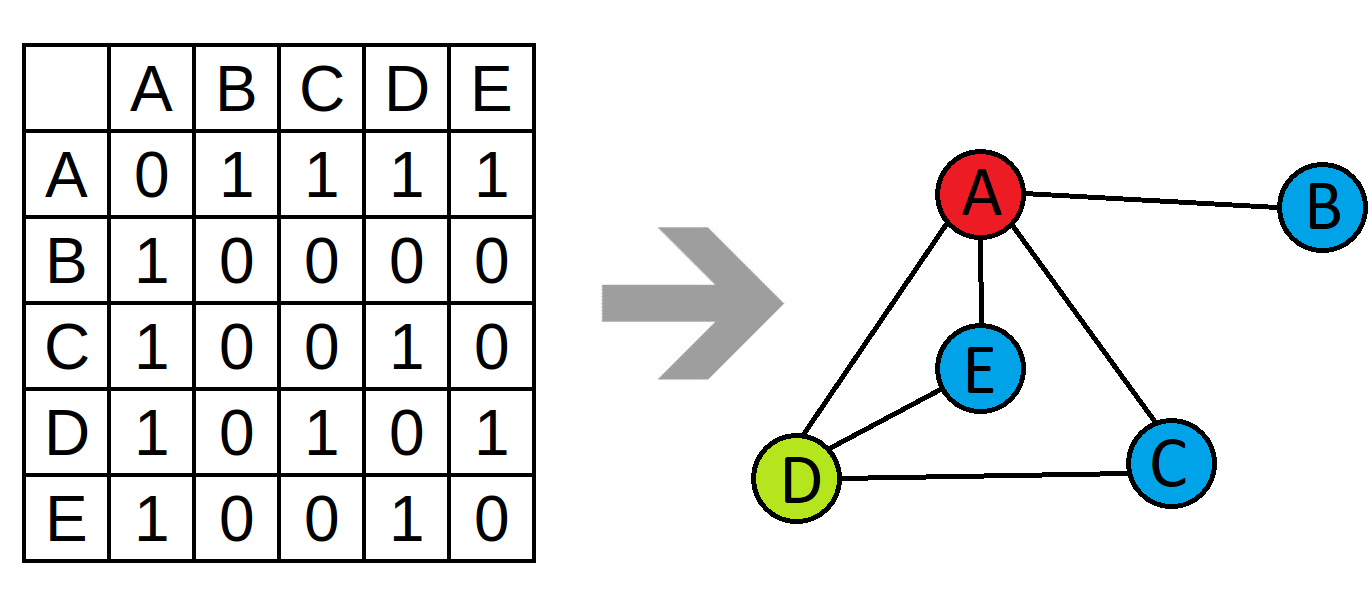
\includegraphics[scale=0.4]{img/colored.png}
\end{frame}

\begin{frame}\frametitle{Algoritmus}
    \emph{Slepé prohledávání se zpětným navracením (backtracking):}
    \begin{itemize}
    \item[$\bullet$] pro CSP (problémy s omezujícími podmínkami) je to metoda \emph{úplná i optimální}
    \item[$\bullet$] navracení implementováno pomocí zásobníku
    \item[$\bullet$] bez vylepšení pomalá metoda pro optimální barvení grafů...
	\end{itemize}
    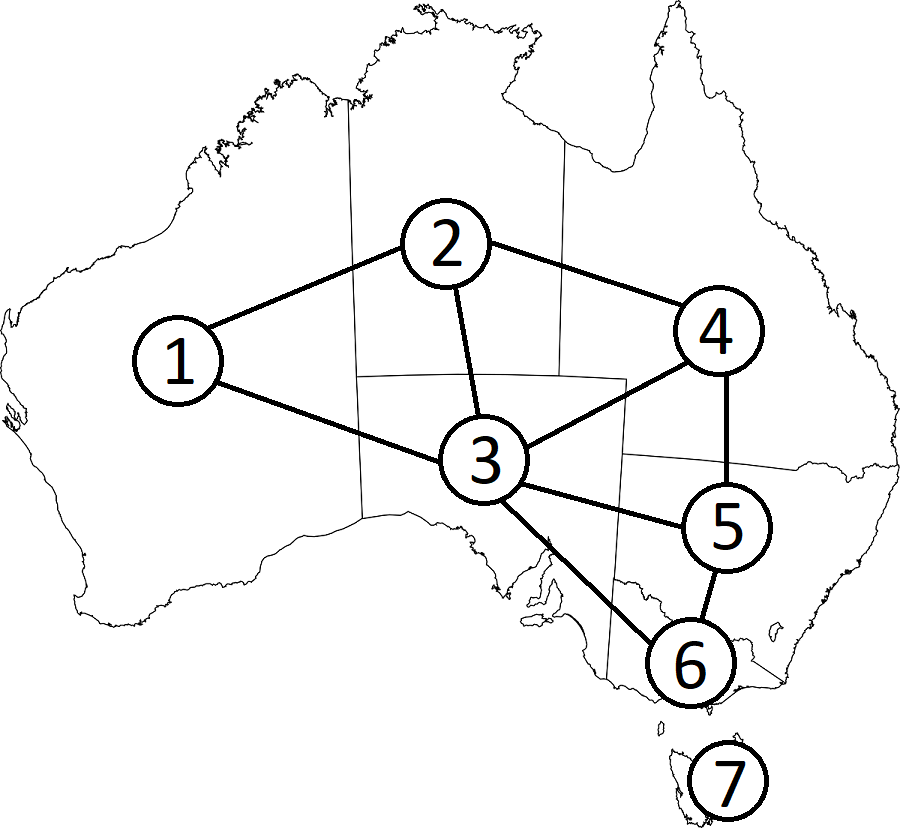
\includegraphics[scale=0.3]{img/australia.png}
    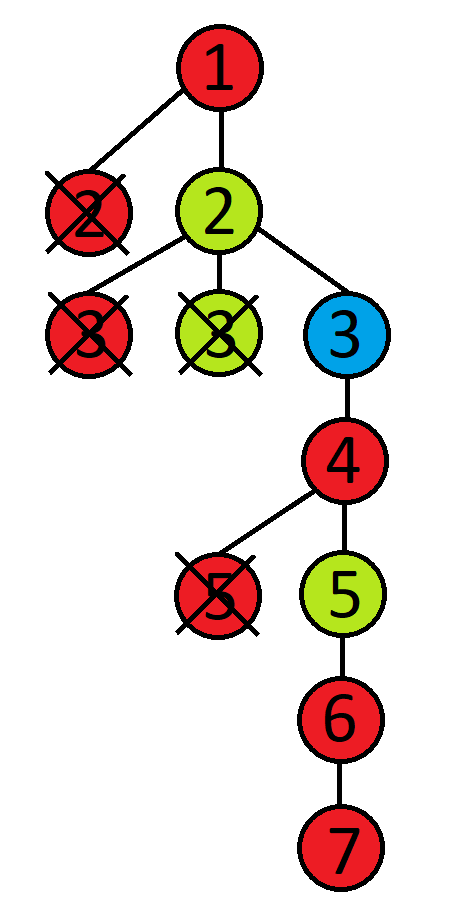
\includegraphics[scale=0.3]{img/backtracking.png}
\end{frame}

\begin{frame}\frametitle{Algoritmus}
    \emph{Kontrola dopředu (forward checking):}
    \begin{itemize}
    \item[$\bullet$] v podstatě rozšíření metody backtracking
    \item[$\bullet$] metoda je schopná dříve odhalit "větve" kombinací barev, které nevedou ke správnému řešení
    \item[$\bullet$] použití množin legálních barev uzlů
    \item[$\bullet$] implementována pomocí rekurze
	\end{itemize}
    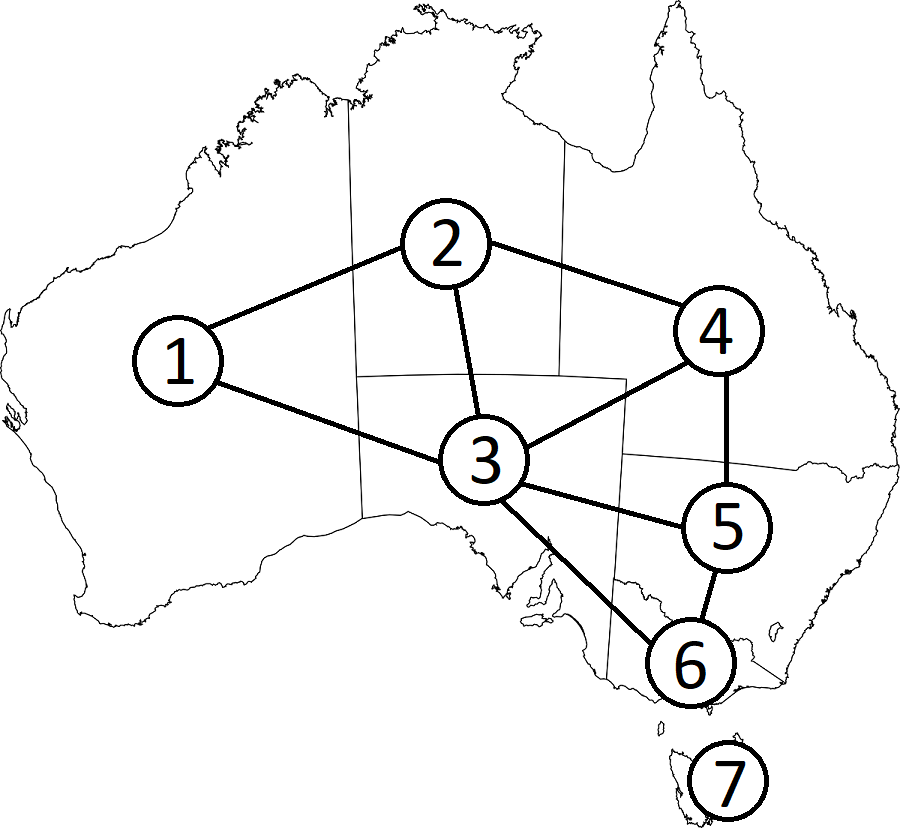
\includegraphics[scale=0.3]{img/australia.png}
    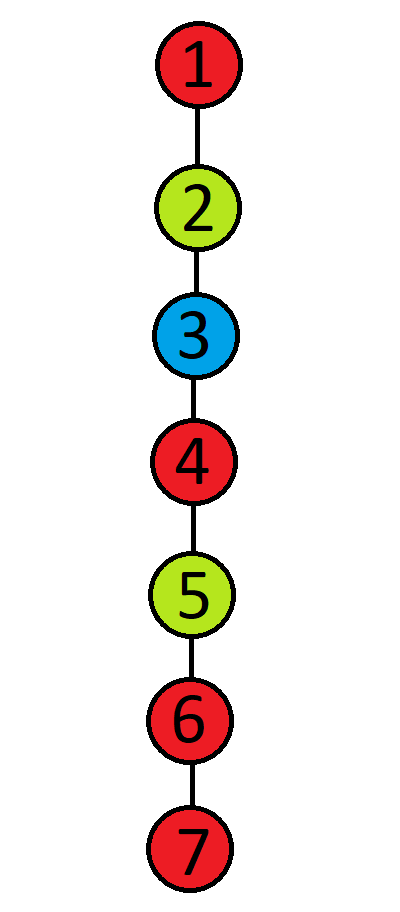
\includegraphics[scale=0.3]{img/fc_tree.png}
    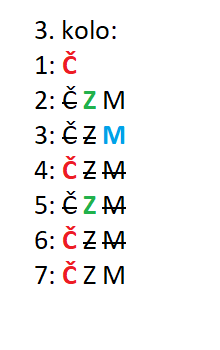
\includegraphics[scale=0.6]{img/fc_sets.png}
\end{frame}

\begin{frame}\frametitle{Struktury}
    \begin{itemize}
	\item[$\bullet$] zvolili jsme matici sousednosti, protože naše úloha řeší i hustě spojené grafy
	\item[$\bullet$] množiny legálních barev implementovány pomocí polí typu bool
	\end{itemize}
    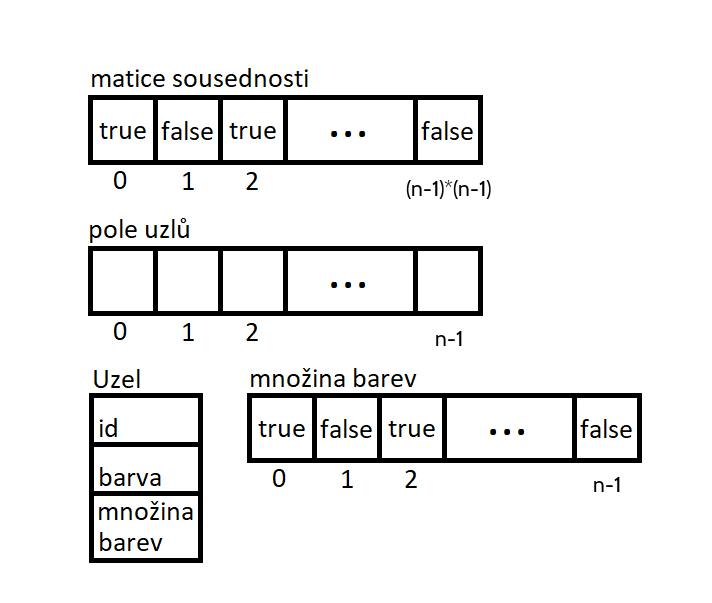
\includegraphics[scale=0.58]{img/structures.png}
\end{frame}

\begin{frame}\frametitle{Časová složitost}
	\begin{itemize}
	\item[$\bullet$] hledání chromatického čísla grafu je \emph{NP-úplný problém}
    \item[$\bullet$] časová složitost metody forward checking: \emph{$O(m^n)$}
    \end{itemize}
    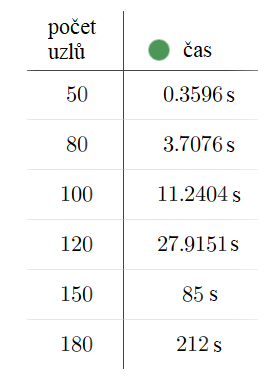
\includegraphics[scale=0.3]{img/complex1.png}
    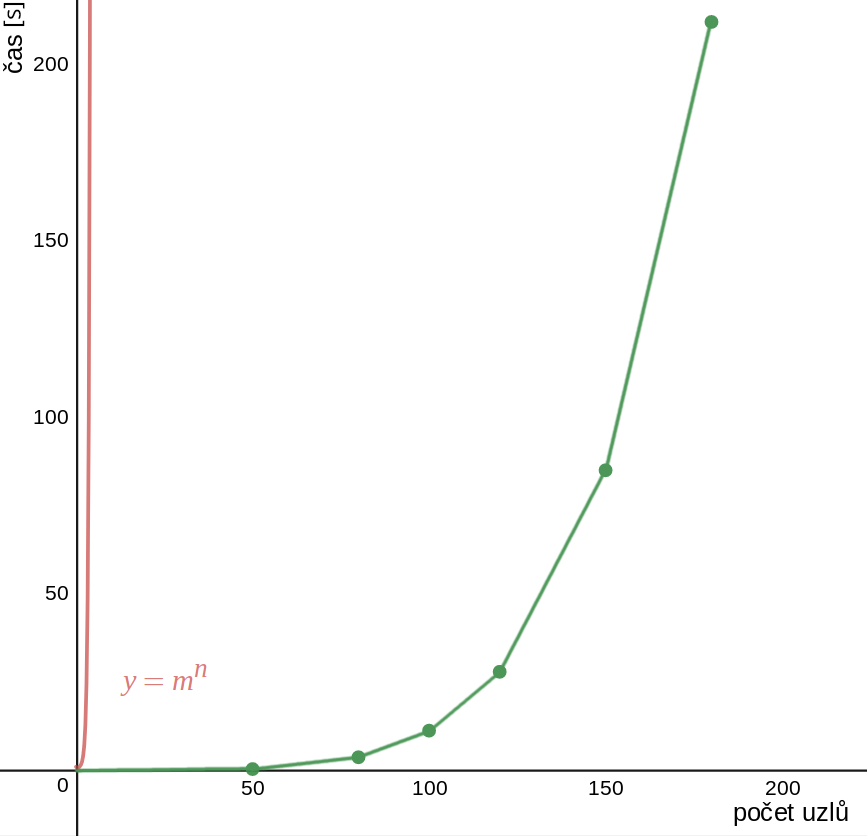
\includegraphics[scale=0.2]{img/complex2.png}
\end{frame}

\begin{frame}\frametitle{Porovnání rychlosti verzí programu}

    \begin{columns}
    \begin{column}{0.5\textwidth}
        \begin{itemize}
        \item[$\bullet$] backtracking
        \item[$\bullet$] forward checking s množinami barev ve dvojsměrném seznamu 
        \item[$\bullet$] forward checking s množinami barev v poli typu bool
        \end{itemize}
    \end{column}
    \begin{column}{0.5\textwidth}
        \begin{center}
         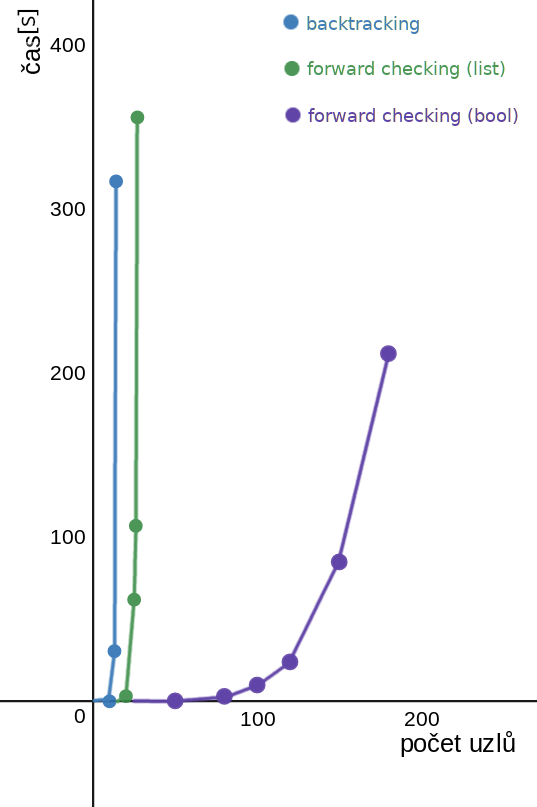
\includegraphics[scale=0.25]{img/compare_alg.png}
         \end{center}
    \end{column}
    \end{columns}
\end{frame}

\begin{frame}\frametitle{Práce v týmu}
    \begin{itemize}
	\item[$\bullet$] pravidelné schůzky, komunikace přes Facebook
	\item[$\bullet$] verzování programu pomocí nástrojů Git a GitHub
	\item[$\bullet$] testování v duchu metody Test-Driven Development
	\end{itemize}
\end{frame}

\bluepage{Děkujeme za pozornost}

\end{document}
